\documentclass[a4paper, 12pt, final, garamond]{book}
\usepackage{cours-preambule}

\raggedbottom

\makeatletter
\renewcommand{\@chapapp}{Ondes -- chapitre}
\makeatother

\begin{document}
\setcounter{chapter}{1}

\chapter{TD~: Interf\'erences \`a deux ondes}
\section{Interférences de 2 ondes sonores frontales}

\begin{minipage}{0.65\linewidth}
    Dans le montage ci-contre, les deux haut-parleurs, notés HP1 et HP2 et
    séparés de la distance $2D$, sont alimentés en parallèle par une même
    tension électrique~: les deux sources sonores émettent donc des vibrations
    $p_1$ et $p_2$ de même pulsation $\w$, même phase à l'origine $\f_0$ et même
    amplitude $P_0$. Les deux ondes arrivent au point M d'abscisse $x$ avec des
    phases différentes et donc interfèrent. On considère que les ondes sonores
    se propagent sans déformation ni atténuation à la célérité $c$ constante.
\end{minipage}
\hfill
\begin{minipage}{0.35\linewidth}
    \begin{center}
        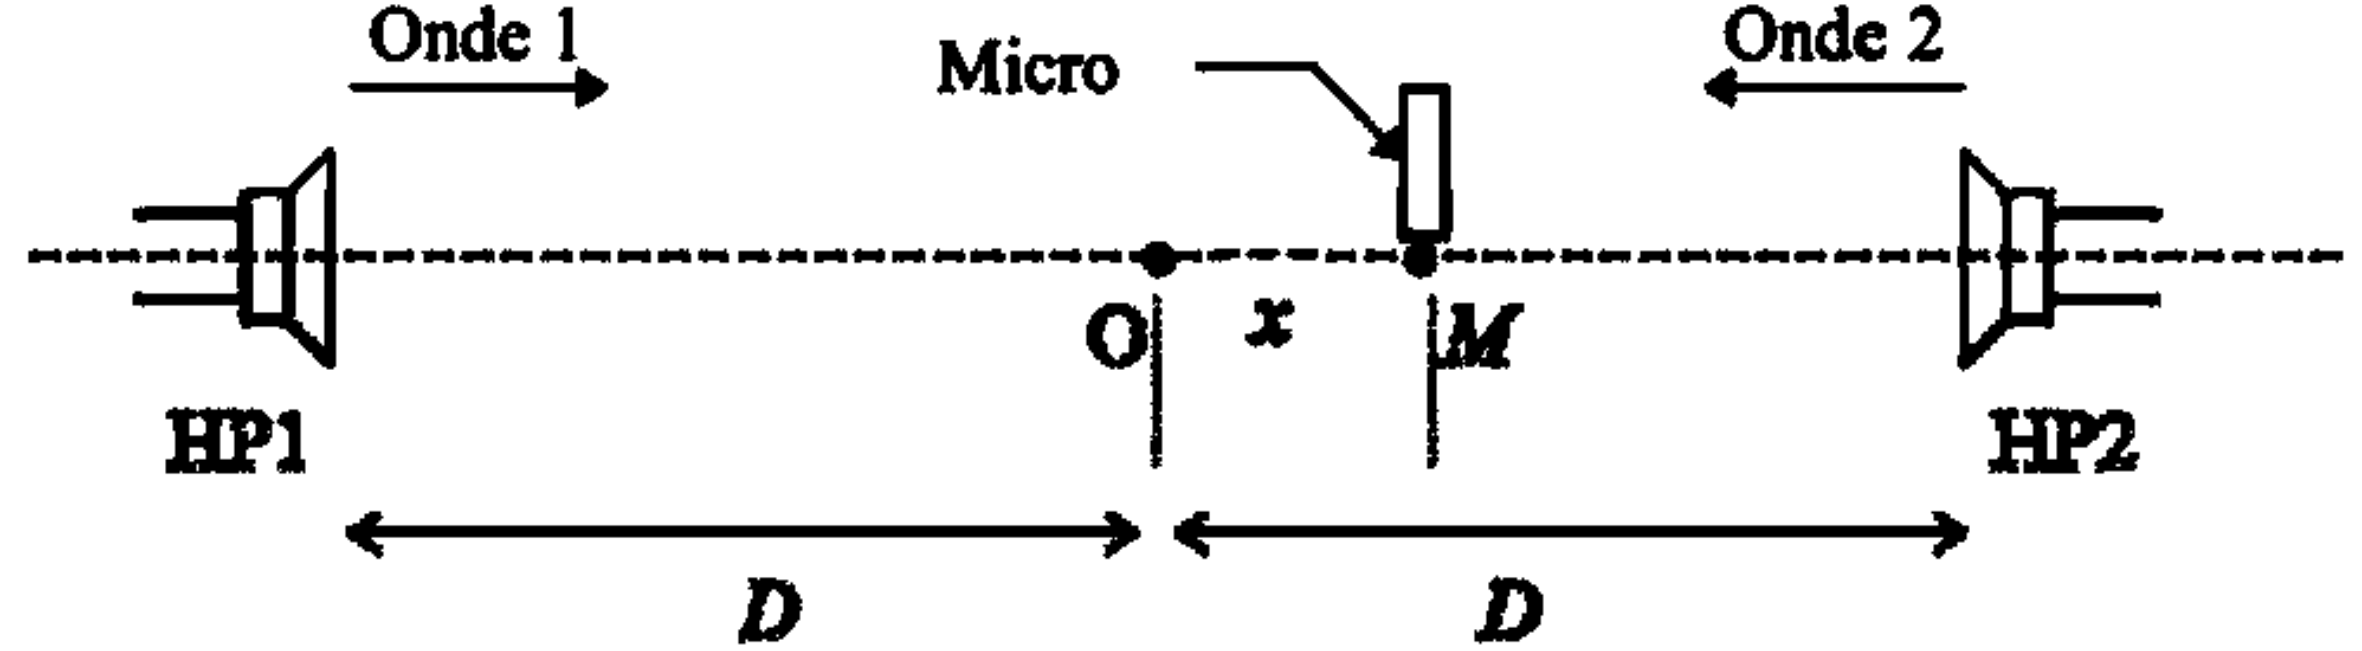
\includegraphics[width=\linewidth]{ondes_front-plain}
    \end{center}
\end{minipage}

\begin{enumerate}
    \item Exprimer le déphasage $\D\f$ au point M entre les ondes issues de HP1
        et HP2.
    \item En déduire l'amplitude de l'onde sonore résultante au point M.
    \item Déterminer les positions $x_n$ pour lesquelles il y a interférences
        constructives au point M.
    \item Exprimer la distance $d$ entre deux maximums successifs d'intensité
        sonore.
    \item Expérimentalement on trouve $d = \SI{21.2}{cm}$ pour une fréquence
        sonore $f = \SI{800}{Hz}$. En déduire la valeur de la célérité du son
        dans l'air pour cette expérience.
\end{enumerate}

\section{Interférences sur la cuve à ondes}

La figure ci-dessous représente une cuve à ondes éclairée en éclairage
stroboscopique. Deux pointes distantes de a frappent la surface de l'eau de
manière synchrone (même fréquence et phase à l'origine), générant deux ondes qui
interfèrent. La figure est claire là où la surface de l'eau est convexe et
foncée là où elle est concave. L'amplitude d'oscillation est plus faible là où
la figure est moins contrastée.

\begin{center}
    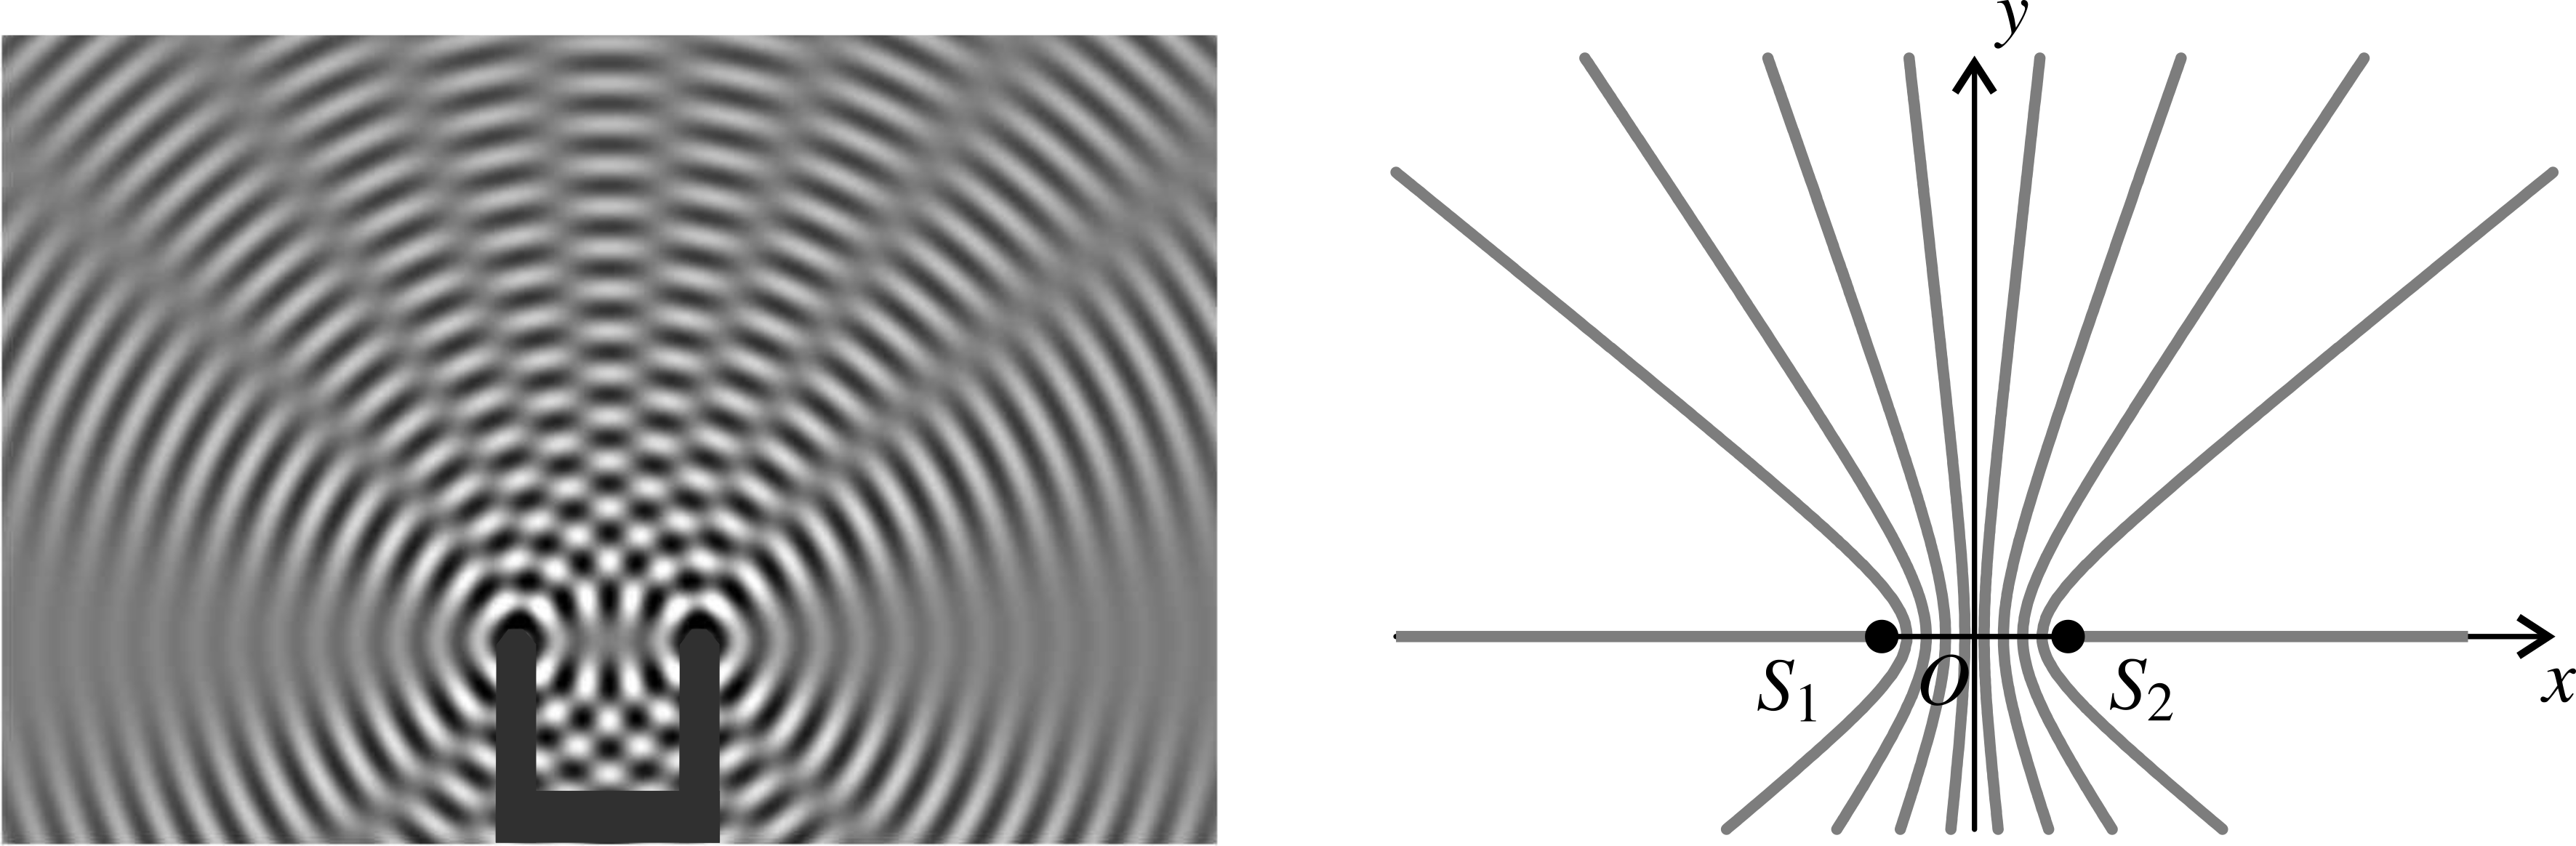
\includegraphics[width=.8\linewidth]{cuve_ondes-plain}
\end{center}

\begin{enumerate}
    \item On suppose pour simplifier que des ondes sinusoïdales partent des deux
        points $S_1$ et $S_2$ où les pointes frappent la surface. En notant
        $\lambda$ la longueur d'onde, donner la condition pour que
        l'interférence en un point M situé aux distances $d_1$ et $d_2$
        respectivement de $S_1$ et $S_2$, soit destructrice. Cette condition
        fait intervenir un entier $m$.

    \item Pour chaque entier $m$ le lieu des points vérifiant cette condition
        est une courbe que l'on appelle dans la suite ligne de vibration
        minimale. Les lignes de vibration minimale sont représentées sur la
        figure de droite~: ce sont des hyperboles. Les parties $x < -a/2$ et $x
        > a/2$ de l'axe (O$x$) sont des lignes de vibration minimale. En déduire
        un renseignement sur $a/\lambda$.

    \item Sur le segment S$_1$S$_2$, quel est l'intervalle de variation de $d_2
        - d_1$~? Déduire de la figure la valeur de $a/\lambda$.
    \item Expliquer pourquoi l'image est bien contrastée au voisinage de l'axe
        (O$y$).
\end{enumerate}

\section{Trombone de \textsc{Kœnig}}

\begin{minipage}{0.70\linewidth}
    Le trombone de \textsc{Kœnig} est un dispositif de laboratoire permettant de
    faire interférer deux ondes sonores ayant suivi des chemins différents. Le
    haut-parleur, alimenté par un générateur de basses fréquences, émet un son
    de fréquence $f = \SI{1500\pm1}{Hz}$. On mesure le signal à la sortie avec
    un microphone branché sur un oscilloscope.
\end{minipage}
\hfill
\begin{minipage}{0.30\linewidth}
    \begin{center}
        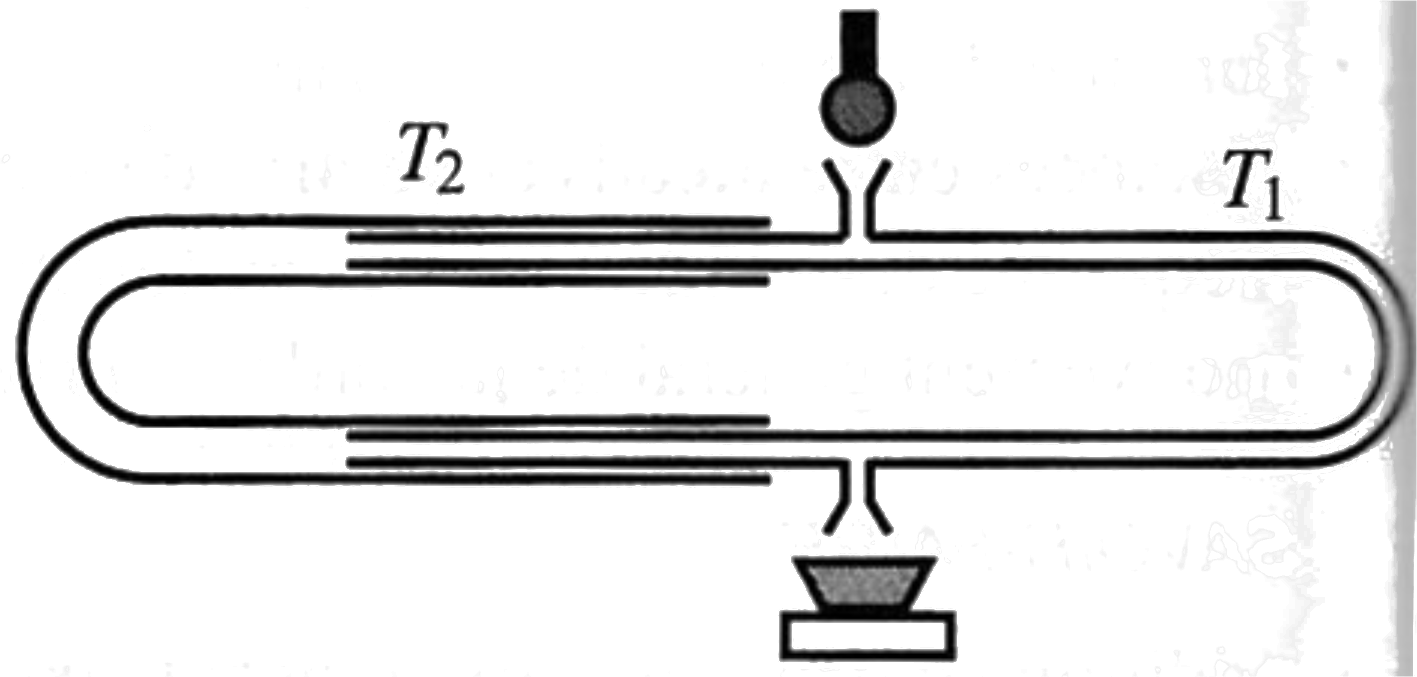
\includegraphics[width=\linewidth]{keonig-plain_white}
    \end{center}
\end{minipage}

\begin{enumerate}
    \item Exprimer en fonction de la distance $d$ de coulissage de $T_2$ par
        rapport à $T_1$ le déphasage au niveau de la sortie entre l'onde sonore
        passée par $T_2$ et celle passée par $T_1$.
    \item En déplaçant la partie mobile $T_2$, on fait varier l'amplitude du
        signal observé. On observe que lorsqu'on déplace $T_2$ de $d =
        \SI{11.5\pm0.2}{cm}$, on passe d'un minimum d'amplitude à un autre. En
        déduire la valeur de la célérité du son dans l'air à
        \SI{20}{\degreeCelsius}, température à laquelle l'expérience est faite.
\end{enumerate}

\section{Interférences et écoute musicale}
\begin{minipage}{0.60\linewidth}
    La qualité de l'écoute musicale que l'on obtient avec une chaîne hi-fi
    dépend de la manière dont les enceintes sont disposées par rapport à
    l'auditaire. On dit qu'il faut absolument éviter la configuration représentée
    sur la figure~: présence d'un mur à une «~petite~» distance $D$ derrière
    l'auditaire.
\end{minipage}
\hfill
\begin{minipage}{0.40\linewidth}
    \begin{center}
        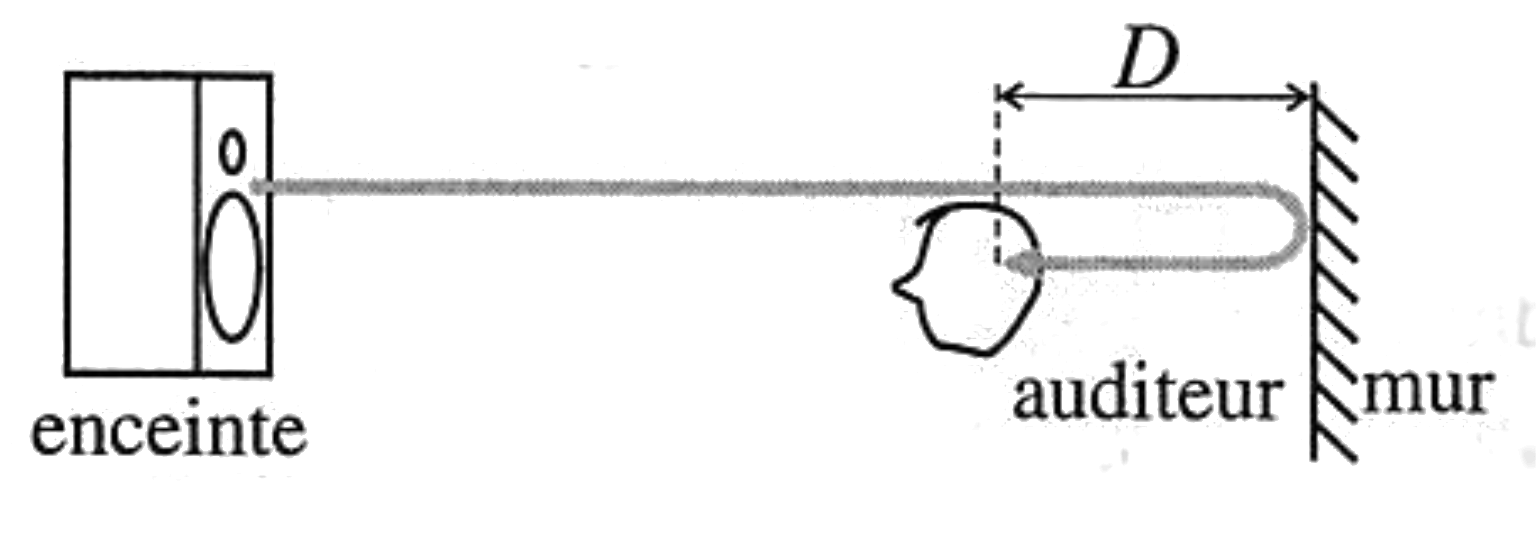
\includegraphics[width=\linewidth]{ecoute_musicale-plain_white}
    \end{center}
\end{minipage}
\bigbreak
Comme représenté sur la figure, l'onde issue de l'enceinte se réfléchit
sur le mur. On note $c = \SI{342}{m.s^{-1}}$ la célérité du son dans l'air.

\begin{enumerate}
    \item Exprimer le décalage temporel $\tau$ qui existe entre les deux ondes
        arrivant dans l'oreille de l'auditaire~: l'onde arrivant directement et
        l'onde réfléchie.
    \item En déduire le déphasage $\D\f$ de ces deux ondes supposées
        sinusoïdales de fréquence $f$. La réflexion sur le mur ne s'accompagne
        d'aucun déphasage pour la vibration acoustique.
    \item Expliquer pourquoi il y a risque d'atténuation de l'amplitude de
        l'onde pour certaines fréquences. Exprimer ces fréquences en fonction
        d'un entier $n$. Quelle condition devrait vérifier $D$ pour qu'aucune de
        ces fréquences ne soit dans le domaine audible. Est-elle réalisable~?
    \item Expliquer qualitativement pourquoi on évite l'effet nuisible en
        éloignant l'auditaire du mur.
\end{enumerate}

\section{Mesure de l'épaisseur d'une lame de verre}

On considère un dispositif de trous d'\textsc{Young} composé de deux trous $T_1$
et $T_2$ séparés d'une distance $a = \SI{100}{\micro m}$. Ce dispositif est
éclairé par une source ponctuelle S monochromatique de longueur d'onde dans
l'air $\lambda = \SI{532}{nm}$ située sur l'axe optique. La figure
d'interférences est observée sur un écran situé à une distance $D =
\SI{1.00}{m}$ du plan des trous. Une lame de verre à faces parallèles
d'épaisseur $e$ inconnue et d'indice $n_v = \num{1.57}$ est positionnée en
sortie du trou $T_1$. L'indice optique de l'air est supposé égal à 1.

\begin{center}
    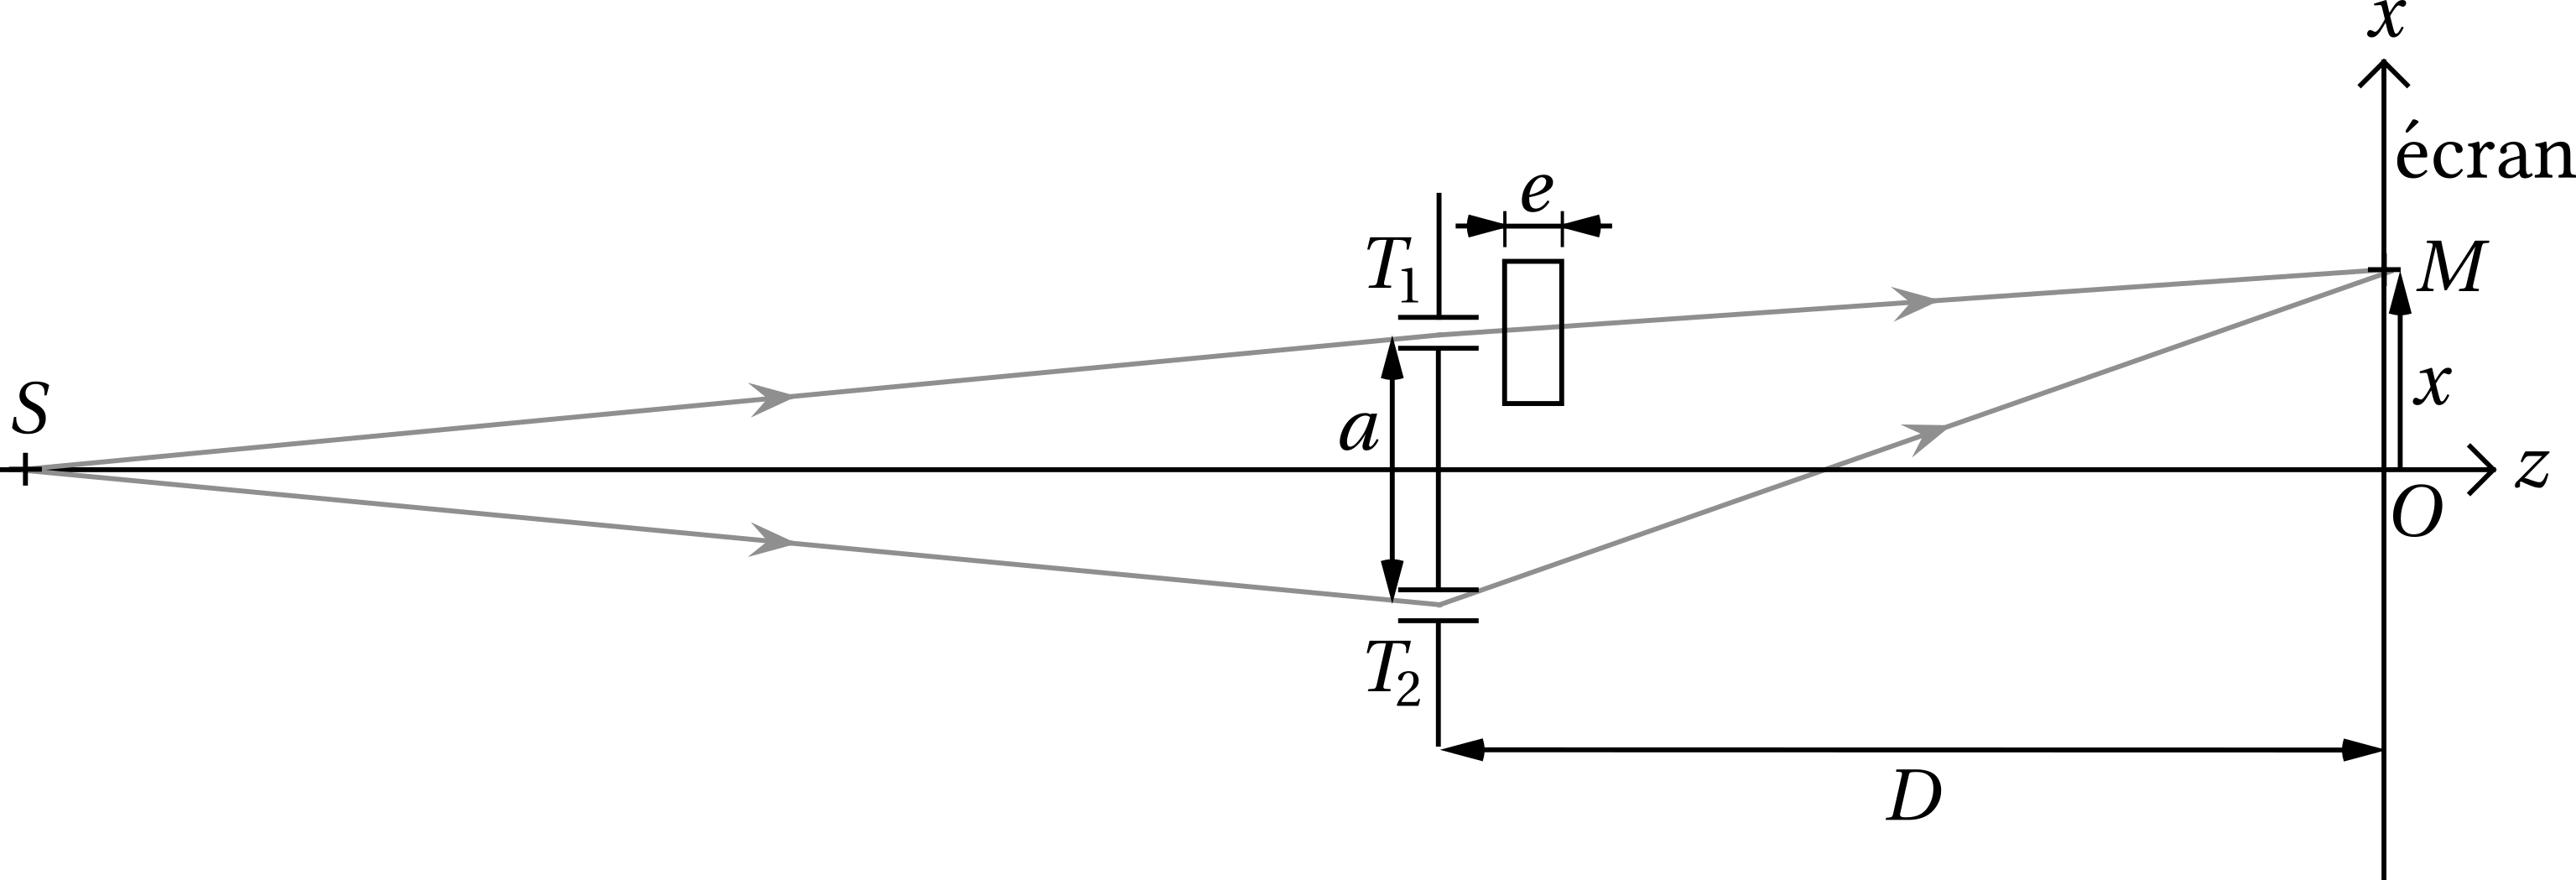
\includegraphics[width=0.8\linewidth]{lame_verre-plain}
\end{center}

\begin{enumerate}
    \item Montrer que la différence de marche $\delta(\Mr)$ en un point M de l'écran
        s'écrit
        \[\delta(\Mr) = \frac{ax}{D} + (n_v - 1)e\]
    \item Déterminer la position $x_c$ sur l'écran de la frange centrale
        correspondant à $\delta(\Mr) = 0$. De quelle distance s'est déplacée
        cette frange par rapport au cas où la lame est absente~?
    \item Exprimer l'épaisseur $e$ de la lame en fonction de $x_c$ , $a$, $n_v$
        et $D$.
    \item Calculer $e$ pour $x_c = \SI{28.5}{cm}$.
    \item Expliquer pourquoi en réalité la position de la frange centrale ne
        peut être connue que modulo l'interfrange $i$. Qu'est-ce que cela
        implique sur $e$~? L'expérience vous paraît-elle réalisable~?
\end{enumerate}

\section{Contrôle actif du bruit en conduite}

\begin{minipage}{0.70\linewidth}
    On s'intéresse à un système conçu pour l'élimination d'un bruit in-
    désirable transporté par une conduite. Le bruit est détecté par un premier
    micro dont le signal est reçu par un contrôleur électronique. Le contrôleur,
    qui est le centre du système, envoie sur un haut-parleur la tension adéquate
    pour générer une onde de signal exactement opposé à celui du bruit de
    manière à ce que l'onde résultante au point A (voir figure ci-contre) et
    au-delà de A soit nulle.
\end{minipage}
\hfill
\begin{minipage}{0.30\linewidth}
    \begin{center}
        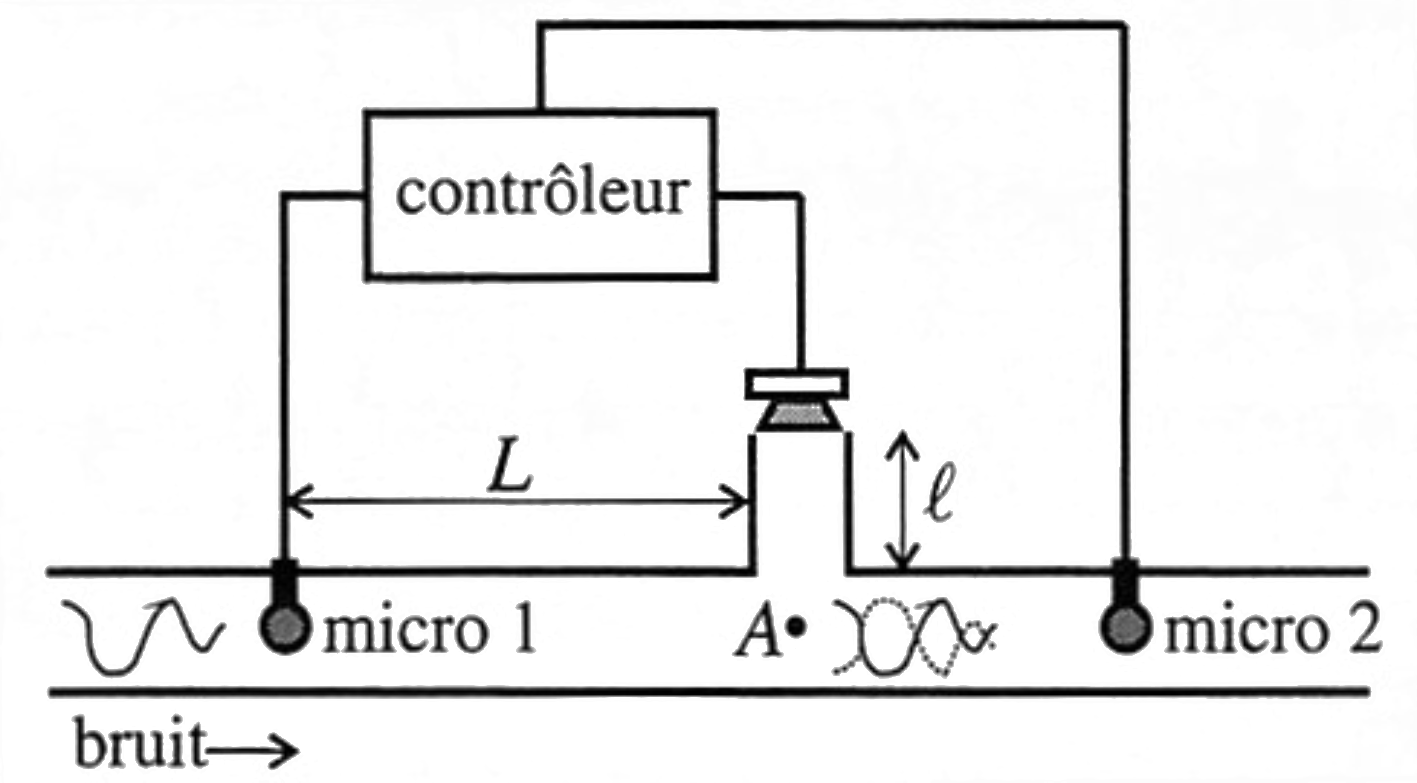
\includegraphics[width=\linewidth]{conduite-plain_white}
    \end{center}
\end{minipage}

\begin{enumerate}
    \item Exprimer, en fonction de $L$, $l$ et de la célérité $c$ du son, le
        temps disponible pour le calcul du signal envoyé sur le haut-parleur.
    \item On suppose le bruit sinusoïdal de pulsation $\omega$. On appelle
        $\f_1$ la phase initiale du signal détecté par le micro 1 et $\f_{\rm
        HP}$ la phase initiale du signal émis par le haut-parleur. Exprimer, en
        fonction de $\omega$, $c$, $L$ et $l$, la valeur que doit avoir $\D\f =
        \f_{\rm HP} - \f_1$
    \item L'onde émise par le haut-parleur se propage dans la conduite dans les
        deux sens à partir de A. Expliquer l'utilité du micro 2.
\end{enumerate}

\section{Mesure de la vitesse du son avec des trous d'\textsc{Young}}

On considère un dispositif composé de deux trous d'\textsc{Young} percés dans un
écran opaque et séparés d'une distance $a = \SI{10.0}{cm}$. Une onde ultrasonore
de fréquence $f = \SI{40}{kHz}$ est envoyée en direction des trous. L'amplitude
de l'onde en sortie des trous est mesurée en utilisant un récepteur qui peut
être translaté suivant un axe (O$x$) parallèle à la direction des trous et situé
à une distance $D = \SI{50.0}{cm}$ du plan des trous. Le dispositif expérimental
est représenté sur la figure 1. Par la suite, les valeurs de $D$ et $a$ sont
supposées connues avec une précision de \SI{1}{mm} et l'incertitude-type sur la
valeur de $f$ est supposée négligeable.

\begin{center}
    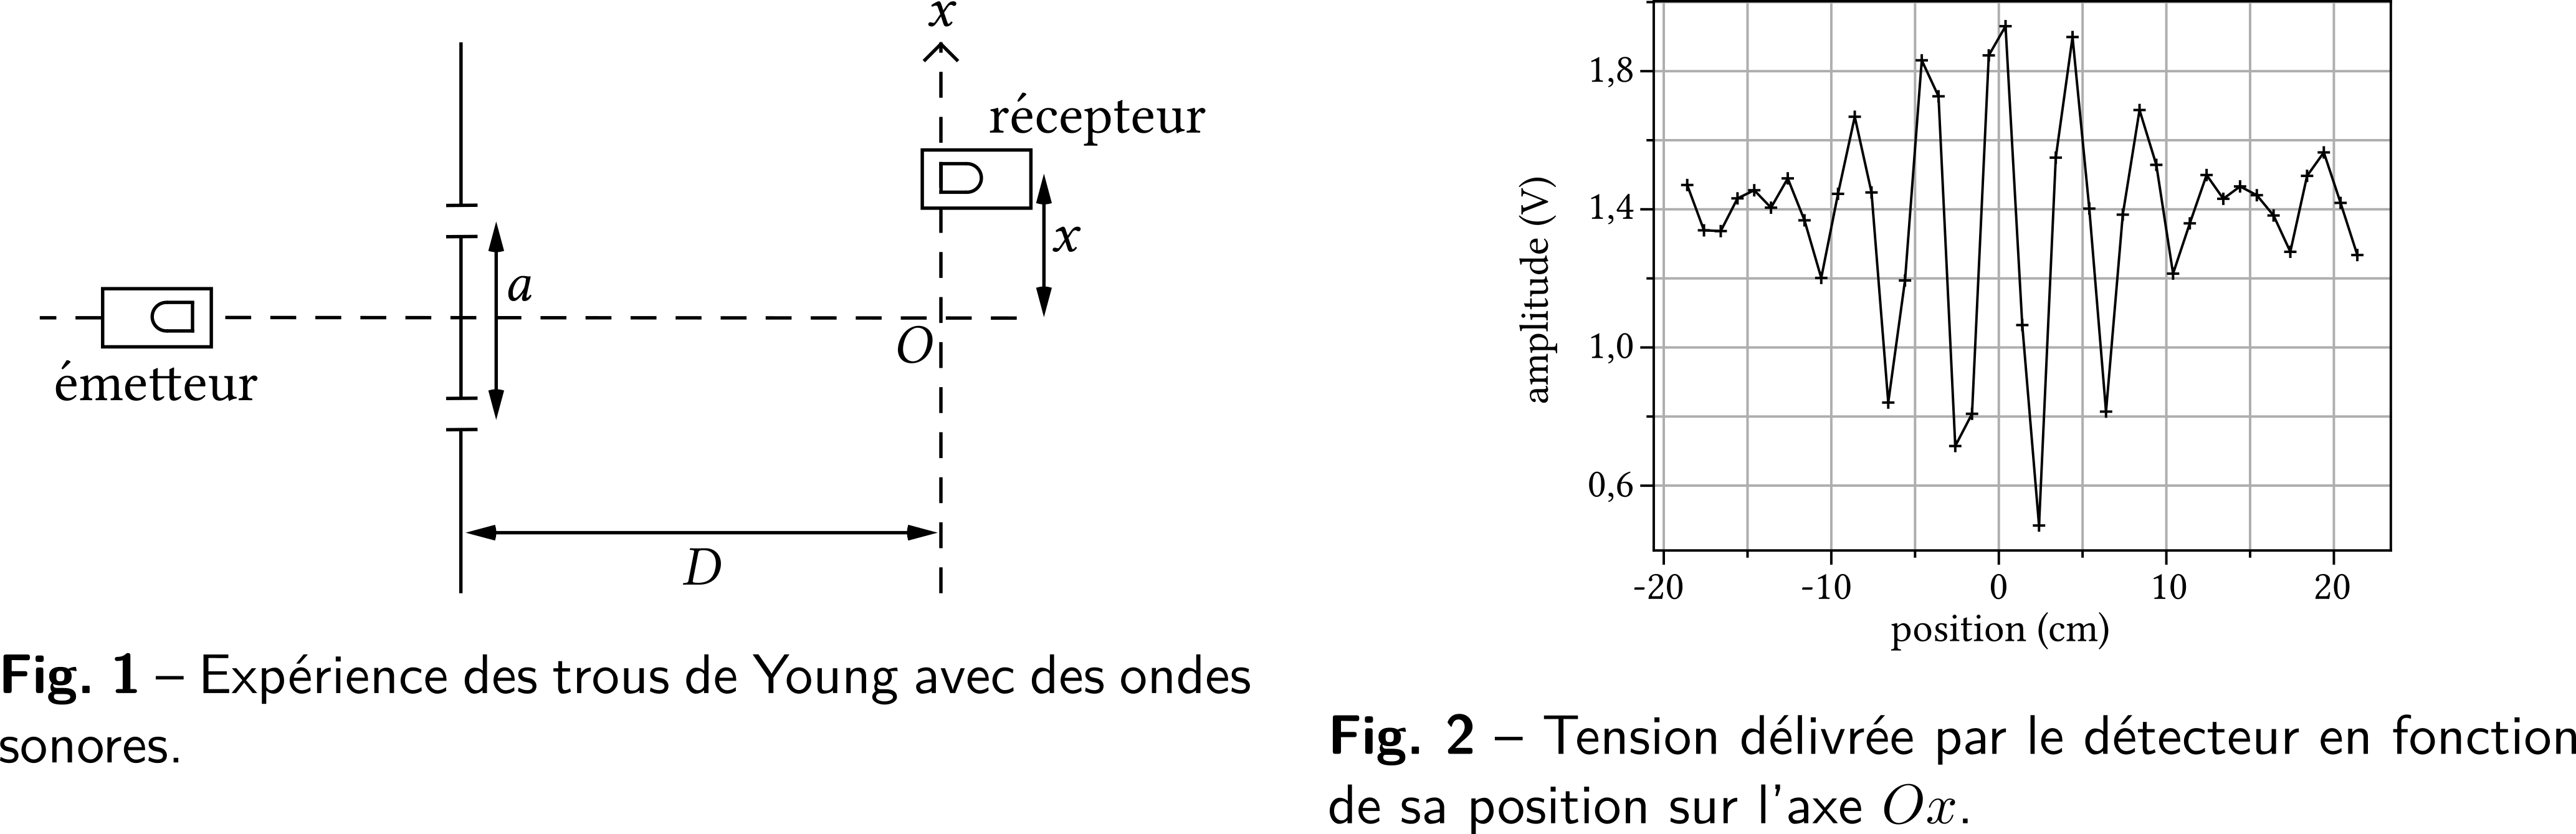
\includegraphics[width=\linewidth]{young_son-plain}
\end{center}

\begin{enumerate}
    \item En supposant que la condition $D \gg a,\,\,x$ est vérifiée, donner
        l'expression de l'interfrange $i$ correspondant à la distance sur l'axe
        (O$x$) entre deux interférences constructives.
\end{enumerate}
Le résultat de la mesure de l'amplitude du signal électrique délivré par le
récepteur en différentes positions sur l'axe (O$x$) est représenté sur la figure
2.
\begin{enumerate}[resume]
    \item À partir de la figure 2, estimer la valeur de l'interfrange ainsi que
        son incertitude-type.
    \item En déduire une estimation de la célérité $c$ du son dans l'air ainsi
        que de son incertitude-type. On néglige toute incertitude sur la
        fréquence $f$.
\end{enumerate}
Un phénomène de diffraction est observé lorsqu'une onde traverse un trou de
rayon $r \approx \lambda$. Le faisceau en sortie du trou présente alors un
demi-angle d'ouverture $\theta$ tel que $\sin(\theta) \approx \lambda/2r$.
\begin{enumerate}[resume]
    \item À partir de la figure 2, estimer l'ordre de grandeur du rayon des
        trous utilisés dans l'expérience.
\end{enumerate}

\section{Interférences ultrasonores sur un cercle}

\begin{minipage}{0.80\linewidth}
    Deux émetteurs E$_1$ et E$_2$ émettent des ondes ultrasonores de même
    fréquence $f = \SI{40}{kHz}$ (ce qui correspond à une longueur d'onde
    $\lambda = \SI{8.5}{nm}$) et en phase. On note O le milieu du segment [E$_1$
    E$_2$] de longueur $a = \SI{4}{cm}$, et (O$x$) l'axe situé sur la médiatrice
    de ce
    segment. On déplace le microphone sur un grand cercle de rayon $R =
    \SI{0.5}{m}$
    et on relève l'évolution de l'amplitude mesurée en fonction de l'angle
    $\theta$ que fait la direction $\vec{\rm OM}$ avec l'axe (O$x$).
\end{minipage}
\hfill
\begin{minipage}{0.20\linewidth}
    \begin{center}
        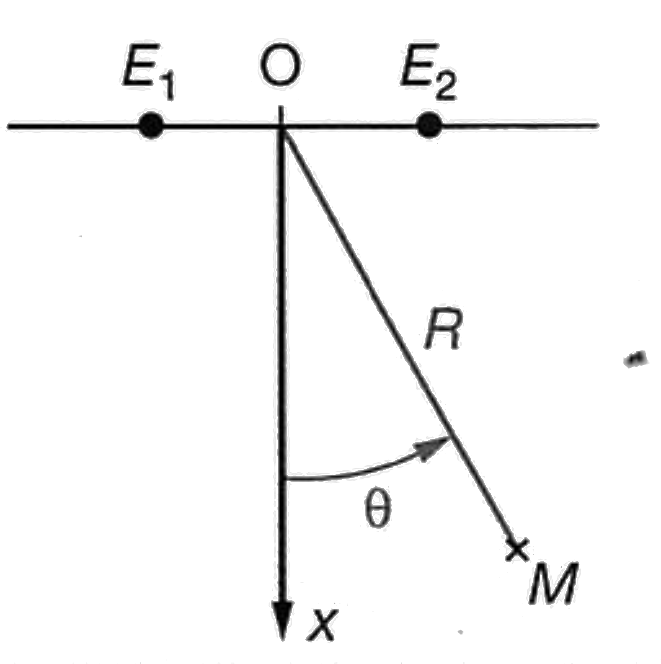
\includegraphics[width=\linewidth]{cercle-plain_white}
    \end{center}
\end{minipage}

\begin{enumerate}
    \item
        \begin{enumerate}
            \item Faire une figure faisant apparaître les points O, E$_1$, E$_2$
                et M, pour un petit angle $\theta$ non nul.
            \item Tracer l'arc de cercle de centre M passant par E$_2$. On note
                H son intersection avec la droite (E$_1$M). Que représente
                E$_1$H~?
            \item Puisque $R \gg a$, on peut assimiler H et le projeté
                orthogonal de E$_2$ sur (E$_1$M). En déduire une expression du
                déphasage entre les ondes reçues en M en fonction de $\theta$,
                $a$ et $\lambda$.
            \item Quelles sont, dans l'intervalle \SIrange{-30}{30}{\degree},
                les valeurs de $\theta$ où on observe un maximum d'amplitude~?
        \end{enumerate}
    \item
        \begin{enumerate}
            \item Sur l'intervalle précédent, quelles sont les positions où un
                minimum d'amplitude est attendu~?
            \item Si les ondes émises ont même amplitude, quelle est la valeur
                minimale d'amplitude pour le signal somme~?
        \end{enumerate}
\end{enumerate}

\end{document}
